\documentclass[11pt]{aghdpl}
% \documentclass[en,11pt]{aghdpl}  % praca w języku angielskim

% Lista wszystkich języków stanowiących języki pozycji bibliograficznych użytych w pracy.
% (Zgodnie z zasadami tworzenia bibliografii każda pozycja powinna zostać utworzona zgodnie z zasadami języka, w którym dana publikacja została napisana.)
\usepackage[english,polish]{babel}

% Użyj polskiego łamania wyrazów (zamiast domyślnego angielskiego).
\usepackage{polski}

\usepackage[utf8]{inputenc}

% dodatkowe pakiety

\usepackage{mathtools}
\usepackage{amsfonts}
\usepackage{amsmath}
\usepackage{amsthm}

% --- < bibliografia > ---

\usepackage[
style=numeric,
sorting=none,
%
% Zastosuj styl wpisu bibliograficznego właściwy językowi publikacji.
language=autobib,
autolang=other,
% Zapisuj datę dostępu do strony WWW w formacie RRRR-MM-DD.
urldate=iso8601,
% Nie dodawaj numerów stron, na których występuje cytowanie.
backref=false,
% Podawaj ISBN.
isbn=true,
% Nie podawaj URL-i, o ile nie jest to konieczne.
url=false,
%
% Ustawienia związane z polskimi normami dla bibliografii.
maxbibnames=3,
]{biblatex}

\usepackage{csquotes}
% Ponieważ `csquotes` nie posiada polskiego stylu, można skorzystać z mocno zbliżonego stylu chorwackiego.
\DeclareQuoteAlias{croatian}{polish}

\addbibresource{bibliografia.bib}

% Nie wyświetlaj wybranych pól.
%\AtEveryBibitem{\clearfield{note}}
% new macro - quotes

\newcommand{\quotes}[1]{``#1''}

% ------------------------
% --- < listingi > ---

% Użyj czcionki kroju Courier.
\usepackage{courier}

\usepackage{listings}
\lstloadlanguages{TeX}

\lstset{
	literate={ą}{{\k{a}}}1
           {ć}{{\'c}}1
           {ę}{{\k{e}}}1
           {ó}{{\'o}}1
           {ń}{{\'n}}1
           {ł}{{\l{}}}1
           {ś}{{\'s}}1
           {ź}{{\'z}}1
           {ż}{{\.z}}1
           {Ą}{{\k{A}}}1
           {Ć}{{\'C}}1
           {Ę}{{\k{E}}}1
           {Ó}{{\'O}}1
           {Ń}{{\'N}}1
           {Ł}{{\L{}}}1
           {Ś}{{\'S}}1
           {Ź}{{\'Z}}1
           {Ż}{{\.Z}}1,
	basicstyle=\footnotesize\ttfamily,
}

% ------------------------

\AtBeginDocument{
	\renewcommand{\tablename}{Tabela}
	\renewcommand{\figurename}{Rys.}
}

% ------------------------
% --- < tabele > ---

\usepackage{array}
\usepackage{tabularx}
\usepackage{multirow}
\usepackage{booktabs}
\usepackage{makecell}
\usepackage[flushleft]{threeparttable}

% defines the X column to use m (\parbox[c]) instead of p (`parbox[t]`)
\newcolumntype{C}[1]{>{\hsize=#1\hsize\centering\arraybackslash}X}


%---------------------------------------------------------------------------

\author{Piotr Konsek i Sebastian Batko}
\shortauthor{P. Konsek, S. Batko}

%\titlePL{Przygotowanie bardzo długiej i pasjonującej pracy dyplomowej w~systemie~\LaTeX}
%\titleEN{Preparation of a very long and fascinating bachelor or master thesis in \LaTeX}

\titlePL{Zastosowanie oprogramowania W3AF w testowanie aplikacji Moodle}
\titleEN{}

%\shorttitlePL{Przygotowanie pracy dyplomowej w~systemie \LaTeX} % skrócona wersja tytułu jeśli jest bardzo długi
%\shorttitleEN{Preparation of a long and fascinating thesis in \LaTeX}

\thesistype{}

\supervisor{}

\degreeprogramme{Informatyka}

\date{2016}

\department{Katedra Informatyki Stosowanej}

\faculty{Wydział Elektrotechniki, Automatyki,\protect\\[-1mm] Informatyki i Inżynierii Biomedycznej}

% TODO:
\acknowledgements{}


\setlength{\cftsecnumwidth}{10mm}

%---------------------------------------------------------------------------
\setcounter{secnumdepth}{4}

\begin{document}

\titlepages

% Ponowne zdefiniowanie stylu `plain`, aby usunąć numer strony z pierwszej strony spisu treści i poszczególnych rozdziałów.
\fancypagestyle{plain}
{
	% Usuń nagłówek i stopkę
	\fancyhf{}
	% Usuń linie.
	\renewcommand{\headrulewidth}{0pt}
	\renewcommand{\footrulewidth}{0pt}
}

\setcounter{tocdepth}{2}
\tableofcontents
\clearpage

\chapter{Wprowadzenie}
\label{cha:wprowadzenie}

Przedstawiony raport ma na celu przetestowania aplikacji Moodle, wykorzystując do tego celu oprogramowanie do testowania W3AF.

%---------------------------------------------------------------------------

\section{Zawartość raportu}
\label{sec:zawartoscPracy}
Struktura raportu jest następująca: 
\begin{itemize}
\item W pierwszym rozdziale opisany został program W3AF, jego konfiguracja oraz użyte pluginy. 
\item W rozdziale drugim omówiona została testowana aplikacja 
\item W rozdziale trzecim prezentujemy testy jakie przeprowadziliśmy na wybranej przez nas aplikacji.
\item W rozdziale czwartym zawarto wnioski 
\end{itemize}

%---------------------------------------------------------------------------

\section{W3AF}
W3AF (Web application attack and audit framework) to aplikacja open-source służąca do testowania bezpieczeństwa aplikacji internetowych Projekt zapewnia skaner podatności oraz narzędzia służące do wydobywania informacji z aplikacji internetowych. Dostarcza niezbędnych informacji o podatnościach na ataki dla wykonania testów penetracyjnych. Aplikacja dostarcza interfejs graficzny do wykonywania testów. Dostępny jest również interfejst tekstowy z linii komend.
\\
W3AF jest podzielony na dwie główne części, rdzeń oraz pluginy. Rdzeń koordynuje prace wszystkich procesów oraz dostarcza featury dostępne dla pluginów, które znajdują podatności oraz wykorzystują je. Pluginy są połączone ze sobą oraz dzielą się informacjami, używając do tego wspólnej bazy wiedzy. Pluginy mogą być podzielone na:
\begin{itemize}
\item Discovery
\item Audit
\item Grep
\item Attack
\item Output
\item Evasion
\item Bruteforce
\end{itemize}

\section{Użyte pluginy}

Do przetestowania aplikacji użyliśmy profilu OWASP\_TOP10, który bada aplikację pod kątem podatności na 10 najczęściej występujacych zagrożeń. Pluginy, które są wykorzystane to:
\begin{itemize}
\item csrf
\item htaccess\_methods
\item webspider
\item blind\_sqli
\item sqli
\item xss
\item buffer\_overflow
\end{itemize}

\section{Konfiguracja}

Niestety na systemie operacyjnym OSX nie jest możliwa praca z W3AF w trybie graficznym. Powodem tego jest występowanie błędu podczas uruchomienia. Spowodowane jest to bugiem w jednej z bibliotek pythona używanych do grafiki. Cała konfiguracja została zatem wykonana za pomocą linii komend. Aby uruchomić W3AF w linii komend, należy uruchomić skrypt a3wf\_console. Po uruchomieniu konsoli i wypisaniu prompta można przystąpić do konfiguracji frameworku. Z poziomu lini komend możemy dowolnie konfigurować działanie programu. Możemy wybrać, które pluginy będą używane, możemy, a nawet musimy skonfigurować cel naszych ataków w opcji target.
\noindent
\begin{minipage}{\linewidth}
\makebox[\linewidth]{
  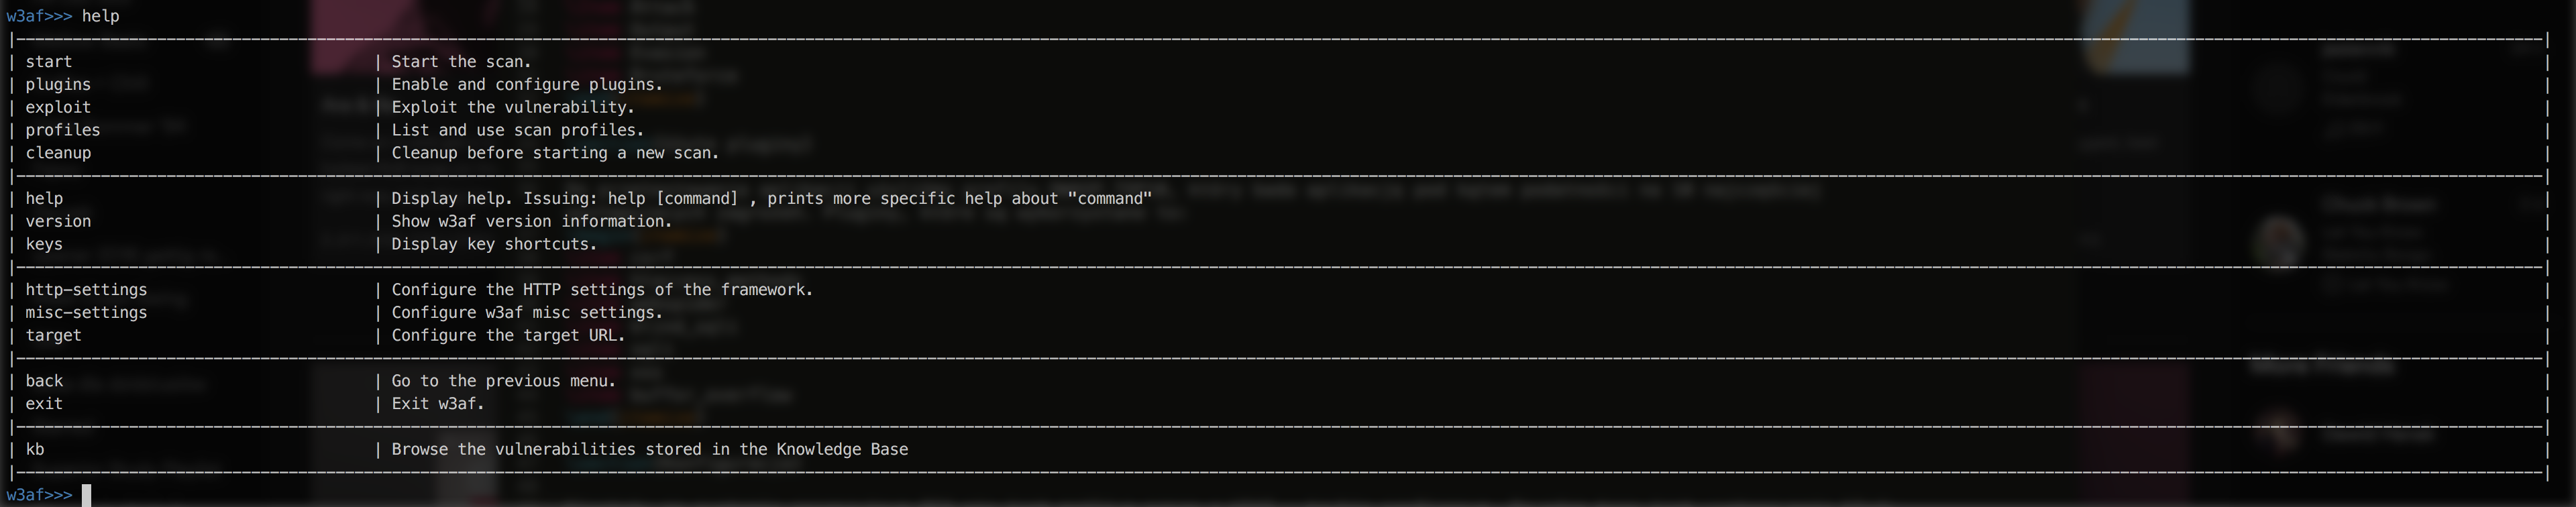
\includegraphics[keepaspectratio=true,scale=0.2]{pictures/options.png}}
\captionof{figure}{Opcje W3AF do wyboru}\label{erd}
\end{minipage}

\noindent
\begin{minipage}{\linewidth}
\makebox[\linewidth]{
  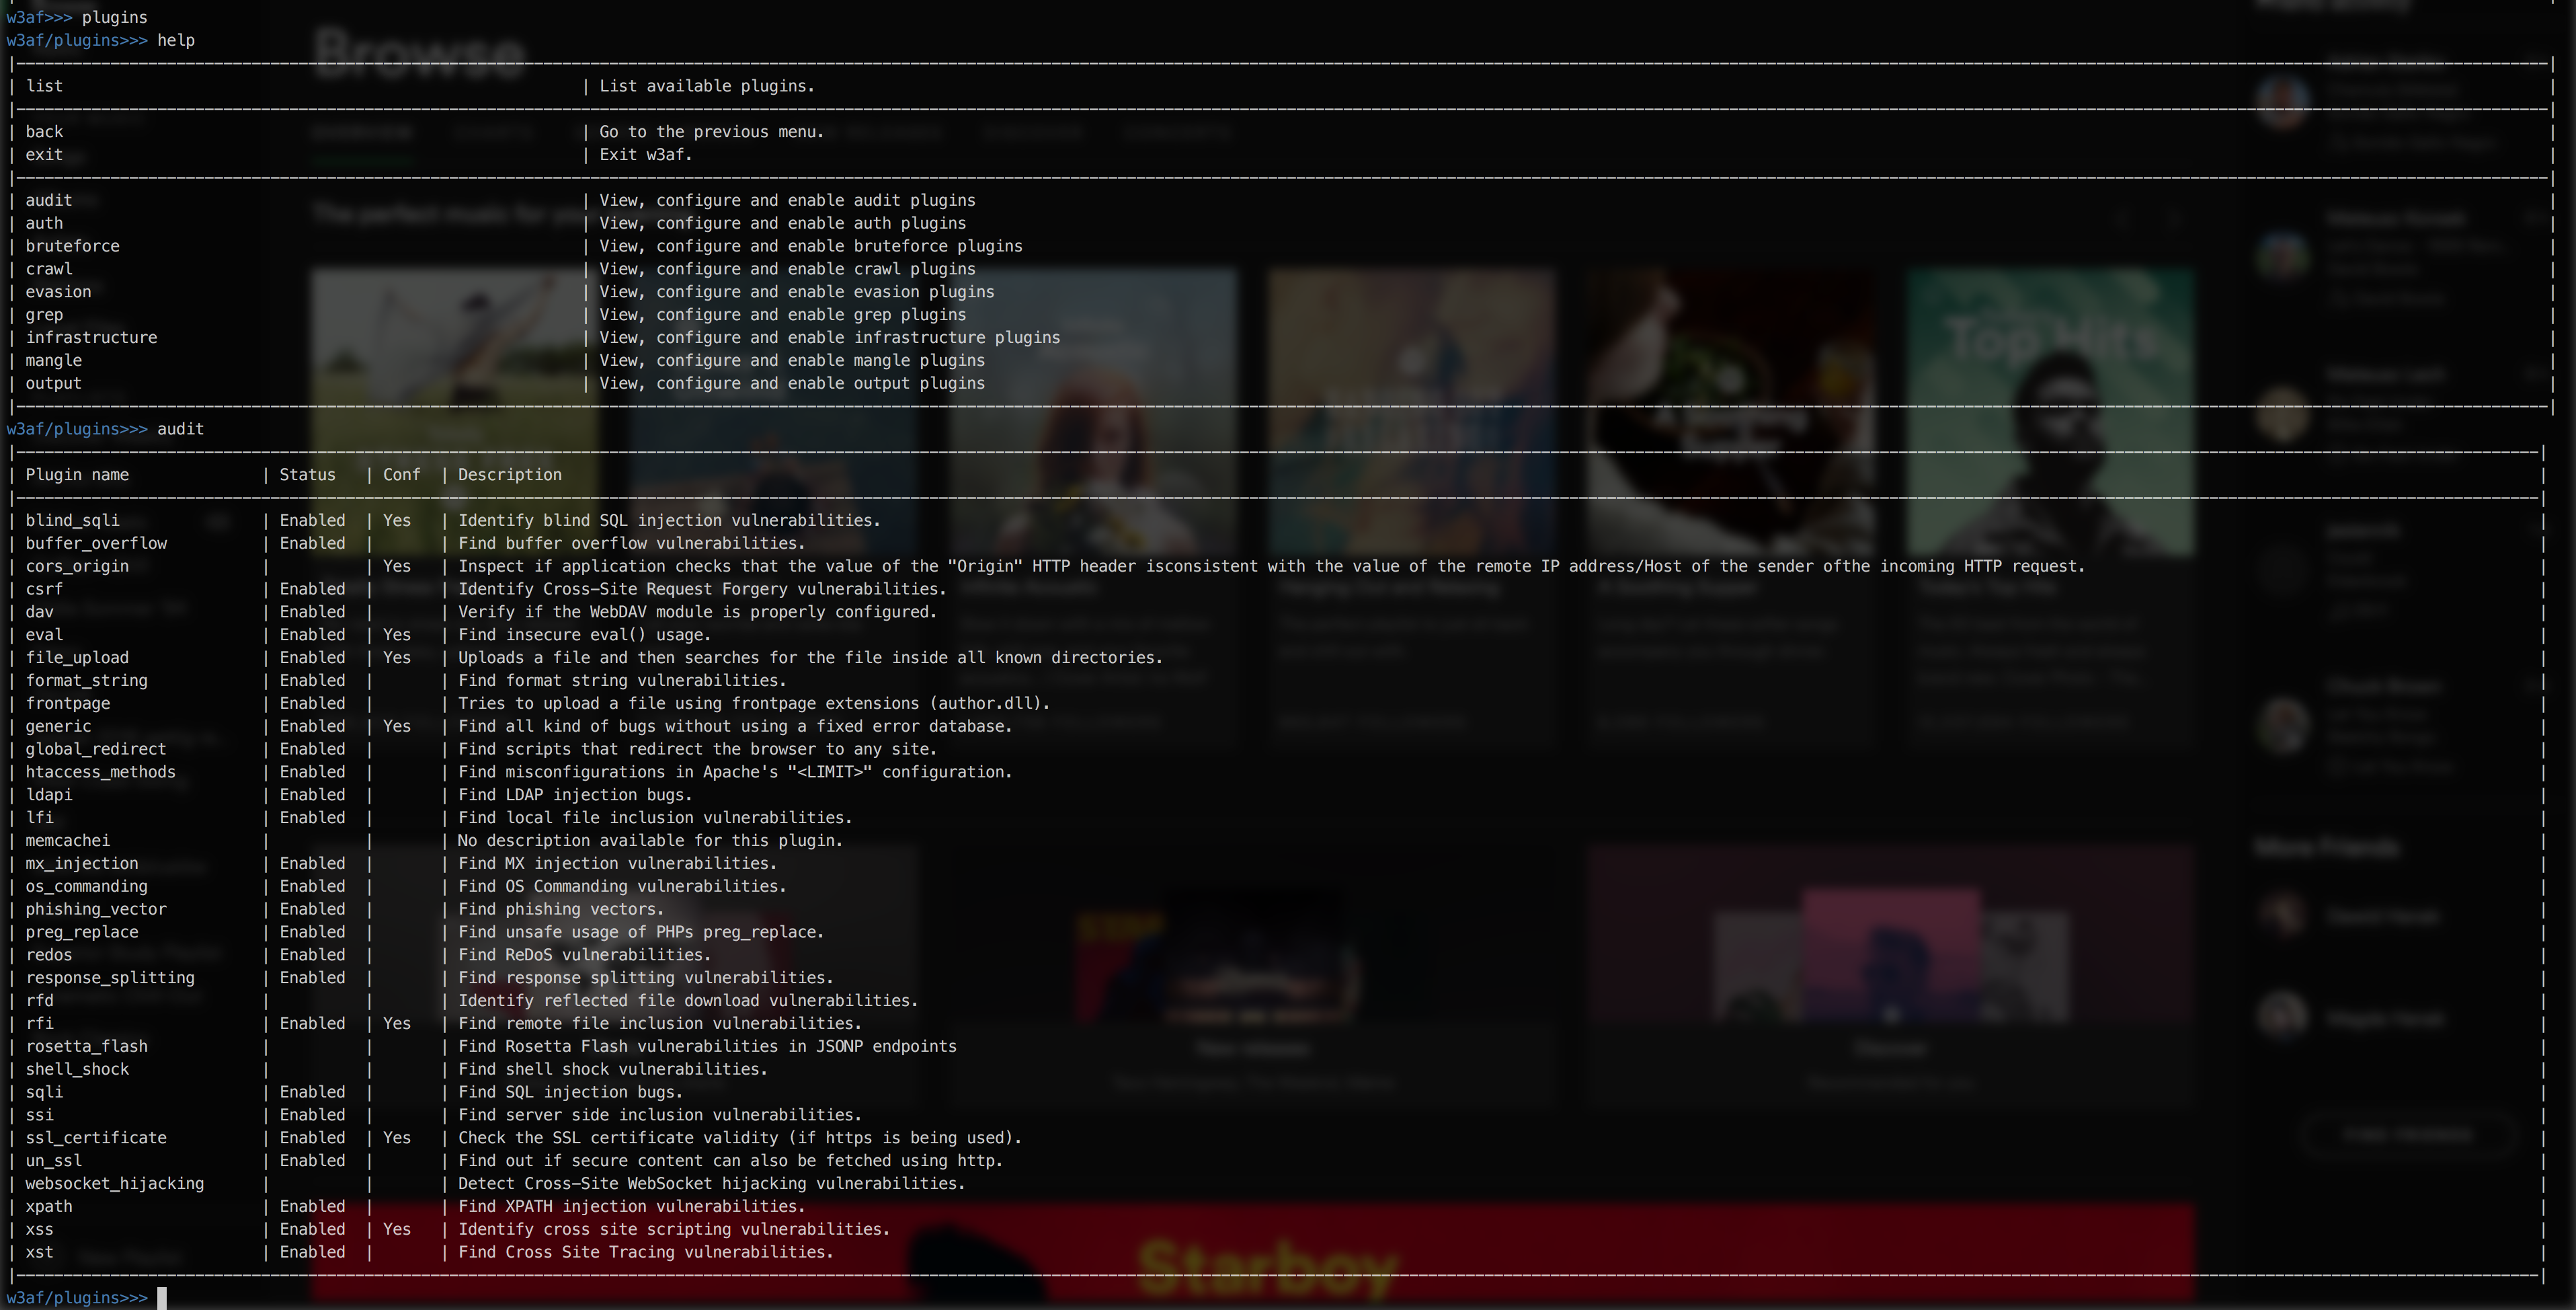
\includegraphics[keepaspectratio=true,scale=0.2]{pictures/plugins.png}}
\captionof{figure}{Różnorodność pluginów do wyboru}\label{erd}
\end{minipage}

\noindent
\begin{minipage}{\linewidth}
\makebox[\linewidth]{
  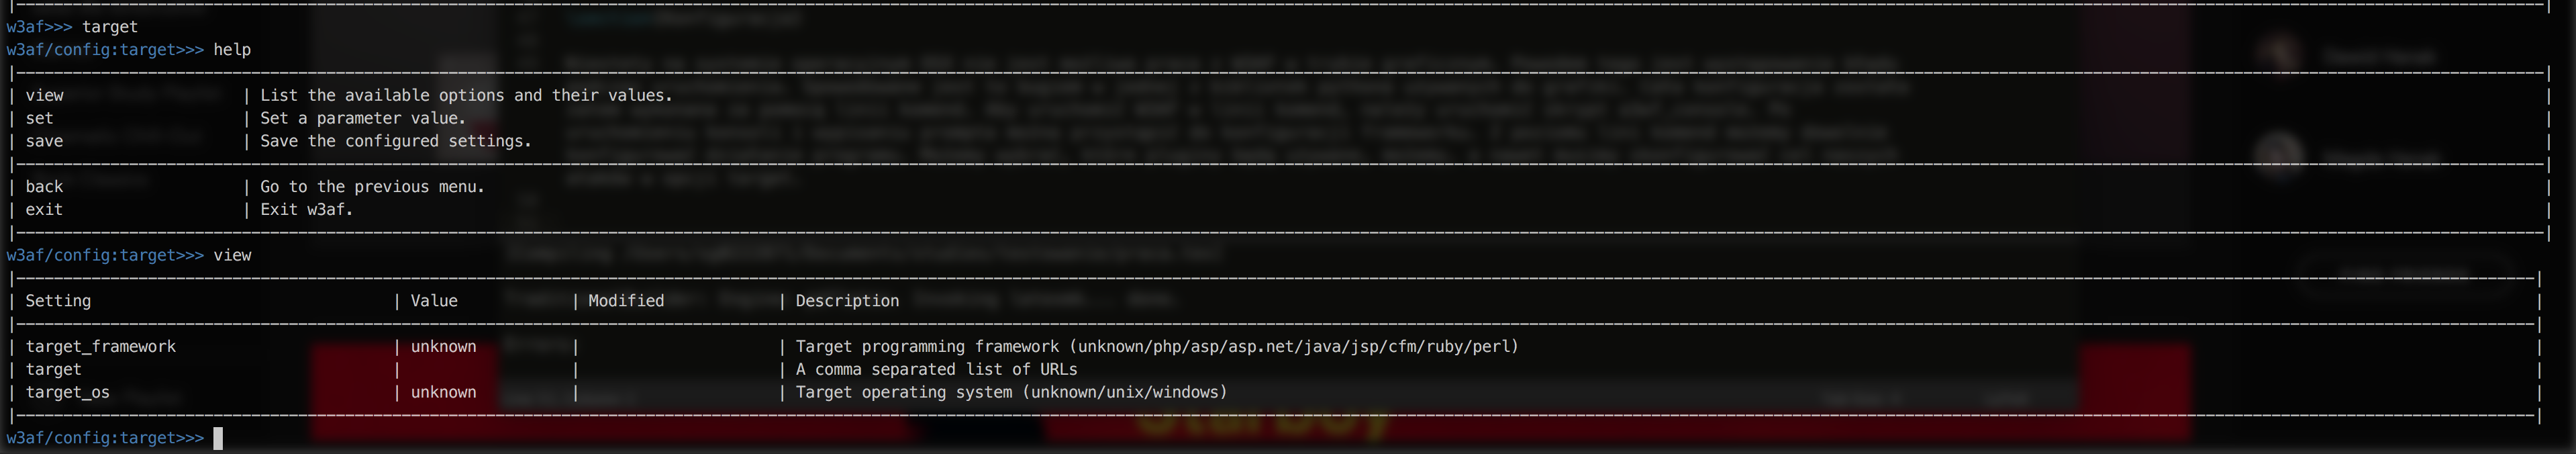
\includegraphics[keepaspectratio=true,scale=0.2]{pictures/target.png}}
\captionof{figure}{Konfiguracja celu ataków}\label{erd}
\end{minipage}

Ostatecznie główne testy przeprowadziliśmy wykorzystując tryb graficzny w3af na systemie Windows. W celu rozpoczęcia pracy należało ustawić URL docelowo testowanej aplikacji wraz z informacją na jakim systemie operacyjnym zostaną wykonane testy, a także technologię w jakiej napisany został testowany kod. Ustawienie tych elementów przedstawia poniższy zrzut:

\noindent
\begin{minipage}{\linewidth}
\makebox[\linewidth]{
  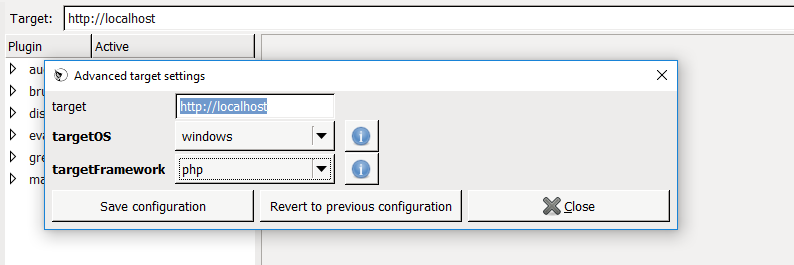
\includegraphics[keepaspectratio=true,scale=0.7]{pictures/w3afconf.png}}
\captionof{figure}{Konfiguracja w3af}\label{erd}
\end{minipage}
\end{enumerate}

W3af oferuje nam szereg różnego rodzaju testów wraz z gotowymi profilami do wyboru, które definiują określony sposób testowania aplikacji. Ten wachlarz możliwości widzimy na zrzucie:

\noindent
\begin{minipage}{\linewidth}
\makebox[\linewidth]{
  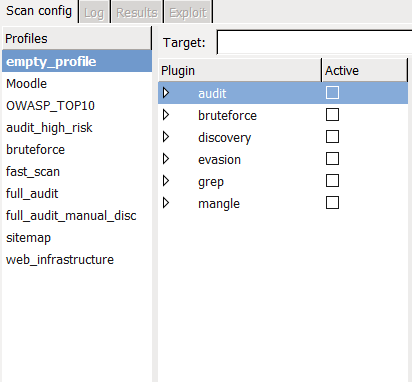
\includegraphics[keepaspectratio=true,scale=0.7]{pictures/w3aftests.png}}
\captionof{figure}{Profile oraz dostępne pluginy}\label{erd}
\end{minipage}
\end{enumerate}






\chapter{Moodle}
\label{cha:moodle}

Moodle to darmowy open-sourcowy program służący do zarządzania kursami uczelnialnymi. System jest napisany w PHP i dytstrybuowany pod licencją GNU. Stworzony z pedagogicznych pobudek, Moodle jest używany do różnorakiej nauki, zdalnej edukacji. Wykorzystując dostosowywalne zarządzanie opcjami, moodle jest używany do tworzenia prywatnych stron oferujących kursy internetowe dla trenerów oraz nauczycieli. Moodle ( akronim od Modular Object-Oriented Dynamic Learing Environment) pozwala na rozszerzanie i dopasowywania środowiska, wykorzystując szeroko dostępne w społeczności pluginy.

Struktura Moodle jest klasyczna dla portalu wymagającego posiadania kont. W Moodle każdy użytkownik posiada osobne konto, do którego przypisana jest jakaś rola. Rolą może być np. administrator, prowadzący kurs albo uczestnik. Żeby stworzyć konto należy się zarejestrować. Moodle jest napisany w całości w PHP, wykorzystuje serwer Apache oraz bazę danych PostgreSQL.

\chapter{Testy}
\label{cha:testy}

Poniżej prezentujemy testy jakie przeprowadzliśmy wraz z ich krótkim opisem oraz niezbędnymi zmianami w kodzie oraz komentarzem odnoszącym się do rezultatów otrzymywanych z w3af.

\section{Click-Jacking}
\begin{enumerate}
\item Opis podatności\\
CLick-Jacking to złośliwa technika nakłaniające użytkowników do klikania w inne rzeczy niż oni sami myślą, że klikają.
Może dojść do potencjalnego ujawnienia poufnych inforamcji lub przejęcia kontroli nad ich komputerem, po kliknięciu na pozornie niewinną stronę. Click-jacking przybiera też formę wbudowanego kodu lub skryptu, który może został wywołany bez wiedzy użytkownika.
\item Zmiany w kodzie\\
Nie były wymagane w przypadku tej podatności.
\item Komentarz\\
W3AF podczas pierwszego uruchomienia, bez zmian w kodzie, wykrył podatność aplikacji Moodle na brak zabezpieczeń przed atakami click-jacking. 
\end{enumerate}

\noindent
\begin{minipage}{\linewidth}
\makebox[\linewidth]{
  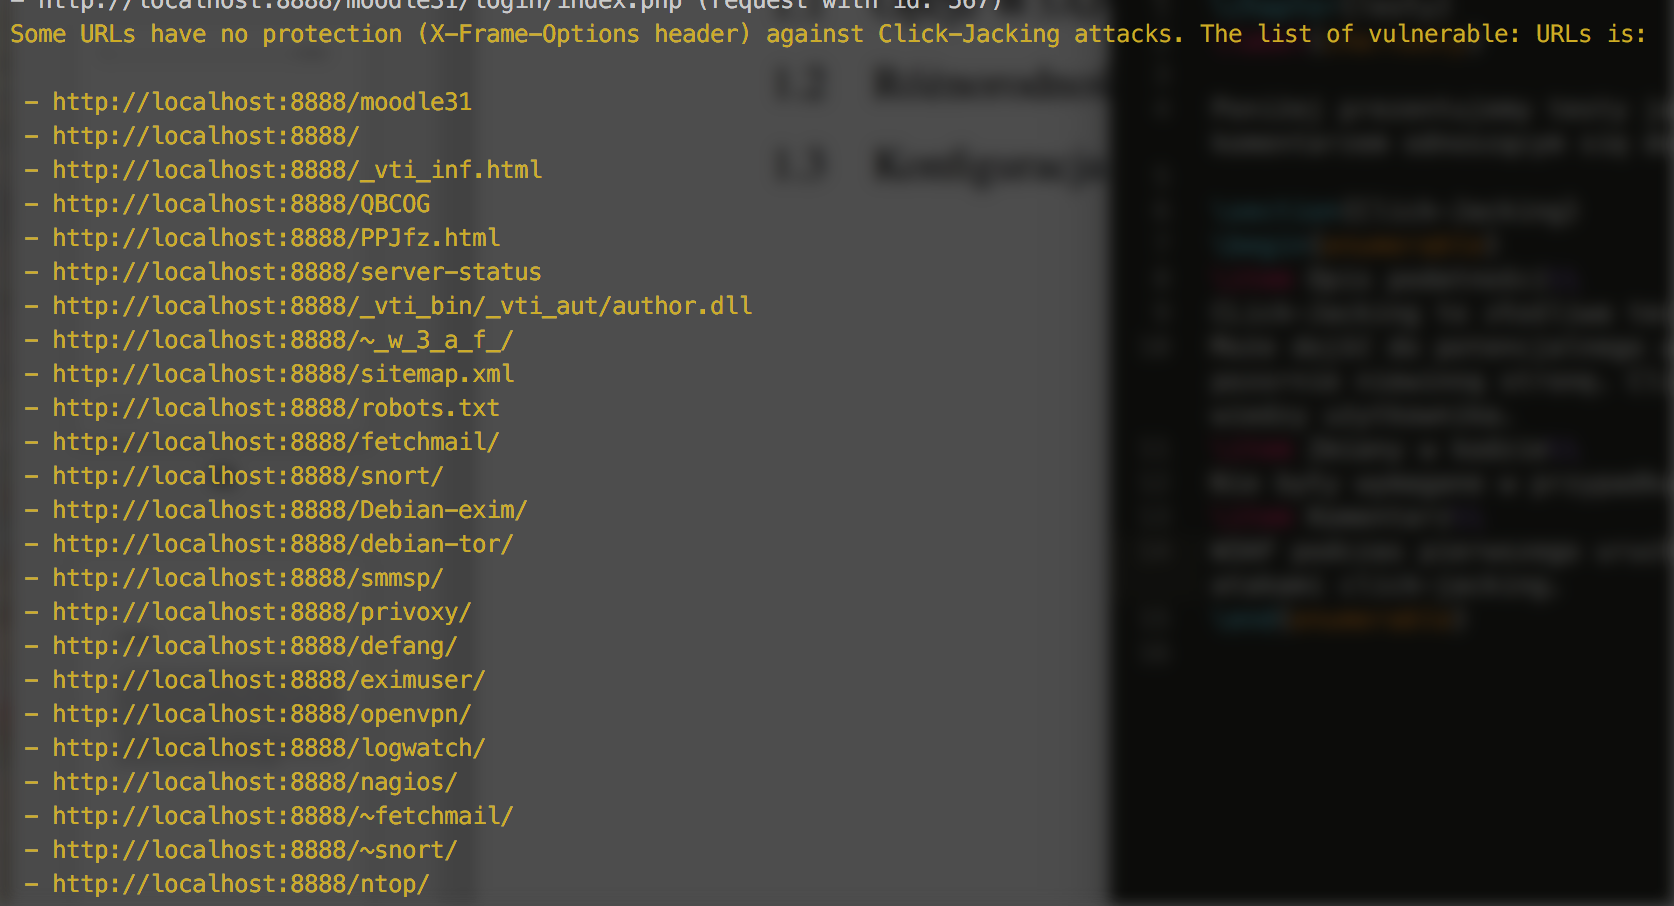
\includegraphics[keepaspectratio=true,scale=0.5]{pictures/clickjacking.png}}
\captionof{figure}{Wyniki W3AF dotyczące clickjackingu}\label{erd}
\end{minipage}

%--------------------------------------

\section{CSRF}
\begin{enumerate}
\item Opis podatności\\
CSRF - metoda ataku na serwis internetowy, która często (m.in. na skutek jednoczesnego wykorzystania) mylona jest z cross-site scripting (XSS) bądź jest uznawana za jej podzbiór. Ofiarami CSRF stają się użytkownicy nieświadomie przesyłający do serwera żądania spreparowane przez osoby o wrogich zamiarach. W przeciwieństwie do XSS, ataki te nie są wymierzone w strony internetowe i nie muszą powodować zmiany ich treści. Celem crackera jest wykorzystanie uprawnień ofiary do wykonania operacji w przeciwnym razie wymagających jej zgody. Błąd typu CSRF dotyczy również serwerów FTP. 
\item Zmiany w kodzie\\
Nie były wymagane w przypadku tej podatności.
\item Komentarz\\
W3AF znalazł podatność na CSRF podczas pierwszego uruchomienia testów:
\noindent
\begin{minipage}{\linewidth}
\makebox[\linewidth]{
  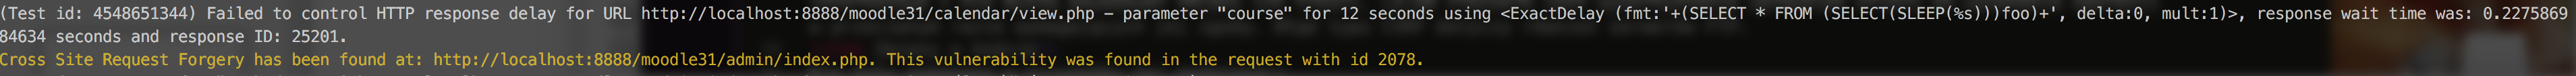
\includegraphics[keepaspectratio=true,scale=0.3]{pictures/csrf.png}}
\captionof{figure}{Wyniki W3AF dotyczące cross site request forgery}\label{erd}
\end{minipage}
\end{enumerate}


%--------------------------------------

\section{SQL injection}
\begin{enumerate}
\item Opis podatności\\
 metoda ataku komputerowego wykorzystująca lukę w zabezpieczeniach aplikacji polegającą na nieodpowiednim filtrowaniu lub niedostatecznym typowaniu danych użytkownika, które to dane są później wykorzystywane przy wykonaniu zapytań (SQL) do bazy danych. Podatne są na nią wszystkie systemy przyjmujące dane od użytkownika i dynamicznie generujące zapytania do bazy danych.
\item Zmiany w kodzie\\
Nie były wymagane w przypadku tej podatności.
\item Komentarz\\
W3AF, a konkretnie plugin blind\_sqli znalazł podatność na CSRF podczas pierwszego uruchomienia testów. Podatne na atak SQL injection są miejsca wpisywania loginu i hasła przez użytkownika.
\noindent
\begin{minipage}{\linewidth}
\makebox[\linewidth]{
  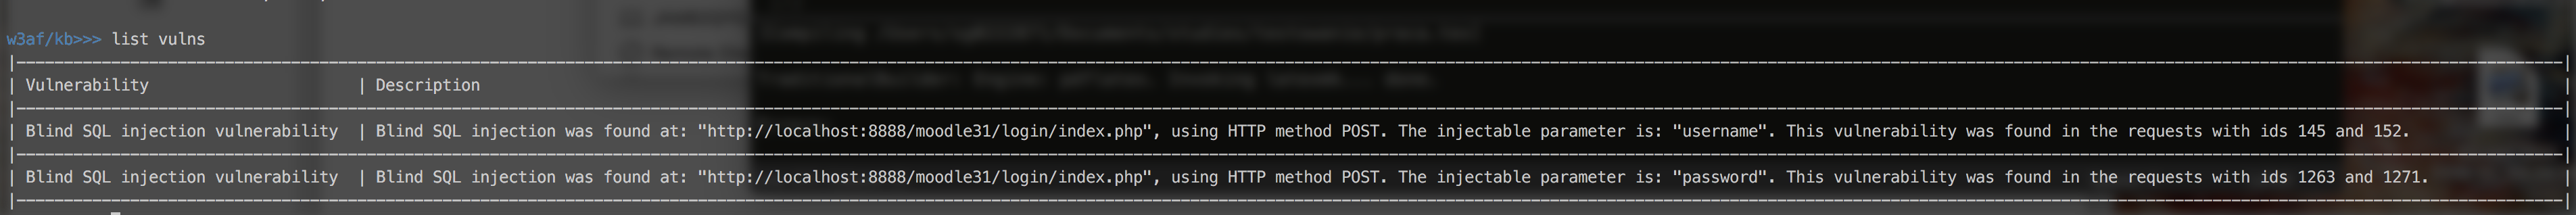
\includegraphics[keepaspectratio=true,scale=0.3]{pictures/sqli.png}}
\captionof{figure}{Wyniki W3AF z bazy wiedzy na temat sql injection}\label{erd}
\end{minipage}
\end{enumerate}

\chapter{Wnioski}

Narzędzie jest bardzo pożytecznym oprogramowaniem. Dla niektórych może się to wydawać trochę dziwne, biorąc pod uwagę fakt, że program jest udostępniany na zasadach licencji open-source. W efekcie prac nad tą aplikacją, powstało oprogramowanie słuażce zabezpieczaniu aplikacji webowych poprzez znajdowanie w nich wszelkiego rodzaju luk bezpieczeństwa.\\

Zaletą narzędzia jest z pewnością mnogich dostępnych pluginów oraz udostępnianych przez nie testów, które można przeprowadzić na dowolnej aplikacji webowej Użytkownik otrzymuje około setki pluginów, które można ze sobą łączyć w dowolny sposób. Każde, dowolne ustawienie konfiguracji można zapisać w postaci profilów. Użytkownik oprogramowania W3AF dostaje out-of-the-box kilka prekonfigurowanych profili z których może korzystać. Wśród tych profili znajduje się między innym OWASP\_TOP10 zawierajcy konfigurację pozwalająca na przetestowanie aplikacji pod kątem 10 najczęściej występujących luk w zabezpieczeniu aplikacji. Lista ta została stworzona przez grupę ekspertów na podstawie badań i ankiet przeprowadzonych wśród topowych dostawców treści internetowych. \\

Dodatkową zaletą aplikacji jest łatwość, z jaką możemy przeglądać zgromadzoną przez program wiedzy w trakcie działania. Minusem jest niestety niska zdolnośc aplikacji do agregacji (łączenia) ze sobą różnych rezultatów. Na szczęście program umożliwia eksport wyników do pliku tekstowego. Do największych wad aplikacji należy jej stabilność oraz brak możliwościu uruchomienia trybu graficznego na sytemie operacyjnym OSX.\\

Naszym zdaniem, używana przez nas aplikacja jest ciekawym narzędziem dostarczającym wiedzę o podstawowych lukach bezpieczeństwa w aplikacji. W3AF może nie jest w stanie ostrzec nas przed bardziej wyrafinowanymi próbami dostępu, lecz jest doskonałym narzędziem wskazującym na podstawowe luki bezpieczeństwa, takiej jak XSS lub clickjacking. Z pewnością, gdyby w3af było rozwijane przez większą liczbę programistów, rezultaty oraz stabilność aplikacji uległaby poprawie.\\

Podsumowując, W3AF jest bardzo ciekawym produktem środowiska open-sourcowego. Nie należy z całkowitą ufnością wierzyć wynikom dostarczanych przez programowanie. Rezultaty jednak mogą być dosyć dobrą wskazówką, gdzie należy szukać podatności aplikacji na ataki.

\listoffigures
\printbibliography

% \chapter{Dodatek}

\end{document}
